\documentclass[letterpaper,12pt]{report} %letterpaper
%\documentclass[letterpaper,12pt]{article} %letterpaper

%\setcounter{secnumdepth}{0}
\usepackage{tikz}
\usetikzlibrary{shapes,arrows}
\usepackage{amsfonts}
\usepackage{amsmath}
\usepackage{amssymb}
\usepackage{colortbl}
\usepackage{float}
\usepackage{algorithm}
\usepackage{algorithmic}
\usepackage{calc}  
\usepackage{enumitem} 
\usepackage{graphicx}
\usepackage{epstopdf}
\usepackage{tikz}
\usetikzlibrary{mindmap, shadows}
\usepackage{metalogo}
\usepackage{verbatim}
\usepackage{dsfont}






\usepackage{xcolor}
\newcommand\ytl[2]{
\parbox[b]{18em}{\hfill{\color{cyan}\bfseries\sffamily #1}~$\cdots\cdots$~}\makebox[0pt][c]{$\bullet$}\vrule\quad \parbox[c]{7.5cm}{\vspace{7pt}\color{red!40!black!80}\raggedright\sffamily #2.\\[7pt]}\\[-3pt]}

\makeatletter% Set distance from top of page to first float
%\setlength{\@fptop}{5pt}
\makeatother

%\input{spanishAlgorithmic} % mi archivo de traducción
\definecolor{orange}{rgb}{1,0.5,0}
\usepackage{hyperref}
\hypersetup{
%%%%--- Options for Acrobat
    bookmarks=true,         % show bookmarks bar?
    unicode=false,          % non-Latin characters in Acrobat's bookmarks
    pdftoolbar=true,        % show Acrobat's toolbar?
    pdfmenubar=true,        % show Acrobat's menu?
    pdffitwindow=false,     % page fit to window when opened
%%%%--- PDF informations
    pdftitle={Introductory Essay},
    pdfauthor={Francisco Richter}, 
    pdfsubject={Simultaneous estimation and selection of species diversification models}, 
    pdfkeywords={},         % list of keywords
%%%%--- Link option
    pdfnewwindow=true,      % links in new window
    colorlinks=true,        % false: boxed links; true: colored links
    linkcolor=blue,         % color of internal links
    citecolor=blue,         % color of links to bibliography
    filecolor=red,         % color of file links
    urlcolor=gray           % color of external links
}

%%%%********************************************************************
% fancy quotes
\definecolor{quotemark}{gray}{0.7}
\makeatletter
\def\fquote{%
    \@ifnextchar[{\fquote@i}{\fquote@i[]}%]
           }%
\def\fquote@i[#1]{%
    \def\tempa{#1}%
    \@ifnextchar[{\fquote@ii}{\fquote@ii[]}%]
                 }%
\def\fquote@ii[#1]{%
    \def\tempb{#1}%
    \@ifnextchar[{\fquote@iii}{\fquote@iii[]}%]
                      }%
\def\fquote@iii[#1]{%
    \def\tempc{#1}%
    \vspace{1em}%
    \noindent%
    \begin{list}{}{%
         \setlength{\leftmargin}{0.1\textwidth}%
         \setlength{\rightmargin}{0.1\textwidth}%
                  }%
         \item[]%
         \begin{picture}(0,0)%
         \put(-15,-5){\makebox(0,0){\scalebox{3}{\textcolor{quotemark}{``}}}}%
         \end{picture}%
         \begingroup\itshape}%
 %%%%********************************************************************
 \def\endfquote{%
 \endgroup\par%
 \makebox[0pt][l]{%
 \hspace{0.8\textwidth}%
 \begin{picture}(0,0)(0,0)%
 \put(15,15){\makebox(0,0){%
 \scalebox{3}{\color{quotemark}''}}}%
 \end{picture}}%
 \ifx\tempa\empty%
 \else%
    \ifx\tempc\empty%
       \hfill\rule{100pt}{0.5pt}\\\mbox{}\hfill\tempa,\ \emph{\tempb}%
   \else%
       \hfill\rule{100pt}{0.5pt}\\\mbox{}\hfill\tempa,\ \emph{\tempb},\ \tempc%
   \fi\fi\par%
   \vspace{0.5em}%
 \end{list}%
 }%
 
 \setcounter{secnumdepth}{4}
\setcounter{tocdepth}{3}
\makeatletter
\newcounter {subsubsubsection}[subsubsection]
\renewcommand\thesubsubsubsection{\thesubsubsection .\@alph\c@subsubsubsection}
\newcommand\subsubsubsection{\@startsection{subsubsubsection}{4}{\z@}%
                                     {-3.25ex\@plus -1ex \@minus -.2ex}%
                                     {1.5ex \@plus .2ex}%
                                     {\normalfont\normalsize\bfseries}}
\newcommand*\l@subsubsubsection{\@dottedtocline{3}{10.0em}{4.1em}}
\newcommand*{\subsubsubsectionmark}[1]{} 
 
 \makeatother
 %%%%********************************************************************


\textwidth=440pt 
\textheight=670pt 
\headheight=1pt
\topmargin=-1cm
\DeclareMathAlphabet{\mathcal}{OMS}{cmsy}{m}{n}
\usepackage{tocbibind}
\usepackage{theorem}
%\newtheorem{propo}{{\sc Proposici—n}}
\newcommand{\argmax}{\operatornamewithlimits{argmax}}



%%%%%%%%%%%%%%%%%%%


%%%--- Header & Footer ---%%%
% 
% 
  \usepackage{fancyhdr}
    \fancyhead[L]{%
      \begin{picture}(.1,.1)
        \put(400,-4.7){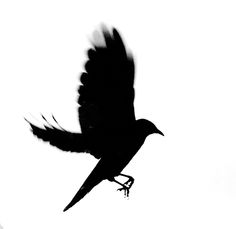
\includegraphics[width=1.3cm]{Pictures/bird.jpg}}
      %  \put(0,3.7){\includegraphics[width=0.5cm]{imagenes/estrellas.png}}
        %\put(10,0){\footnotesize{\leftmark}}
      \end{picture}}
    \fancyhead[R]{}
%%%%-Movie within the Margin
    \fancyfoot[R]{ 
%%%-LSO Line at Footrule
      %\begin{picture}(.1,.1)
        %\put(-10,-28){\includegraphics[width=0.4cm]{estrella}}
    %  \end{picture}
%%%-Small movies :-)
      \ifthenelse{\thepage > 3}{
        \ifthenelse{\thepage < 173}{
          \ifthenelse{\isodd{\thepage}}
            {}
            {
              \ifthenelse{\thepage = 86}
              {}
                         }
        }
      }
    }
    \fancyfoot[C]{\Large \thepage}
    
    
        \renewcommand{\headrulewidth}{0.4pt}
    \renewcommand{\footrulewidth}{0.4pt}
    \pagestyle{fancy}

%%%%%%%%%%%%%%%%%%%%



%\setcounter {section} {2}


\begin{document}

\begin{titlepage}

\newcommand{\HRule}{\rule{\linewidth}{0.5mm}} % Defines a new command for the horizontal lines, change thickness here

\center % Center everything on the page
 
%----------------------------------------------------------------------------------------
%	HEADING SECTIONS
%----------------------------------------------------------------------------------------

\includegraphics[scale=0.2]{Pictures/logo.jpg}\\[0.1cm] 
\textsc{\LARGE University of Groningen}\\[1.5cm] % Name of your university/college

\textsc{\large Johann Bernoulli Institute for Mathematics and Computer Science}\\[0.5cm] % Major heading such as course name
\textsc{\large Groningen Institute for Evolutionary Life Sciences}\\[0.5cm] % Minor heading such as course title

%----------------------------------------------------------------------------------------
%	TITLE SECTION
%----------------------------------------------------------------------------------------

\HRule \\[0.4cm]
{ \huge \bfseries Simultaneous estimation and selection of species diversification models}\\[0.4cm] % Title of your document
\HRule \\[1.5cm]
 
%----------------------------------------------------------------------------------------
%	AUTHOR SECTION
%----------------------------------------------------------------------------------------

\begin{minipage}{0.4\textwidth}
\begin{flushleft} \large
\emph{Author:}\\
Francisco Richter % Your name
\end{flushleft}
\end{minipage}
~
\begin{minipage}{0.4\textwidth}
\begin{flushright} \large
\emph{Supervisors:} \\
Prof. Dr. Ernst C. Wit\\ % Supervisor's Name
Prof. Dr. Rampal S. Etienne
\end{flushright}
\end{minipage}\\[4cm]

% If you don't want a supervisor, uncomment the two lines below and remove the section above
%\Large \emph{Author:}\\
%John \textsc{Smith}\\[3cm] % Your name

%----------------------------------------------------------------------------------------
%	DATE SECTION
%----------------------------------------------------------------------------------------

{\large \today}\\[3cm] % Date, change the \today to a set date if you want to be precise

%----------------------------------------------------------------------------------------
%	LOGO SECTION
%----------------------------------------------------------------------------------------

% Include a department/university logo - this will require the graphicx package
 
%----------------------------------------------------------------------------------------

%\vfill % Fill the rest of the page with whitespace

\end{titlepage}
\newpage
\thispagestyle{empty}
\mbox{}
\newpage
\tableofcontents
\newpage
\thispagestyle{empty}
\mbox{}
\newpage
\chapter{Introduction}
{\color{gray}
 \begin{fquote}[Eduardo Galeano]  Disasters are called natural, as if nature were the executioner and not the victim. \end{fquote} }


Biodiversity, the term used to describe the wide variety of species on Earth, is declining at enormous rates due to human-induced environmental changes. The last time that Earth experienced such high rates of biodiversity loss in a relatively short time was at the end of the Cretaceous period, 65 millon years ago, then most dinosaurs went extinct \cite{wake2008we}. Biodiversity loss, in turn, compromises ecosystem stability and productivity, which negatively impacts the ecosystem services on which human communities depend \cite{tilman2006biodiversity}. \\


%\vspace*{2cm}


%Phylogenetic... blabla... Heal stuff... \\

To conserve biodiversity, we must understand the mechanisms how it comes about and how it is maintained, in assemblages of species, so-called ecological communities. Novel genomic tools make it possible only now to measure and model species in great detail. In the last decade sophisticated methods have been developed that primarily aimed at inferring the evolutionary relatedness of the species (the phylogenetic tree) from DNA sequence data on the basis of models of species diversification. On figure \ref{avian} we can see the phylogenetic tree of the most complete analysis of avian species \cite{jetz2012global}.\\

About 1.7 million species have been identified and given scientific names, but only about $100,000$ of these are popular enough for taxonomist to know them well. There are estimated to be anywhere from 6 to 15 million species on Earth. Many new species are found each year; for instance, 361 new species (mostly insects) were found in the remote rainforest of Borneo from 1999 to 2004 \cite{chivian2008sustaining}. \\

Mathematical and statistical tools have been crucial to generate an understanding on diversification processes \cite{gillman2009introduction}. However there is still a lot to improve. Most of current models have some major shortcomings: they are either too simplistic, too specific or overly complex increasing the dimensionality of the system enormously.\\
% We will briefly review some of them in the next section. \\

% ... All models are wrong.. blabla ... however we can ... \
 
Novel differential geometric approach to statistical methods have been successful implemented on biological data \cite{augugliaro2013differential}\cite{abegaz2013sparse}, and give us a hope to reduce the inferential and computational complexity of the diversification scenario. In this project, we will consider models that account for local interactions and complex ecology information. \\
 
 
This manuscript has been written to be readable for both mathematicians and biologist, as well as a broader audience. Keeping that in mind, in chapter 2 we discuss an overview of the evolutionary diversification process and the ecological mechanism behind it. In chapter 3 we introduce the statistical modeling of the problem step by step. Finally, last tree chapters comment the knowledge utilization of this project, the timeline, and the bibliography respectively. 

%The notation used for the models is included on the appendix. 
%In next chapter we review the current result on the fild as well as describing the... and the biological research questions we will face ... 

%on chapter 3 we describe the mathematical modeling which is going to be applied on this project... blablabla


%Finally we included on the apendix a glosary and the notation used on this chapter, if there is any doubt about any biological or notational concept do not hesitate to go to the appendix to ... 


 \begin{figure}
\centering
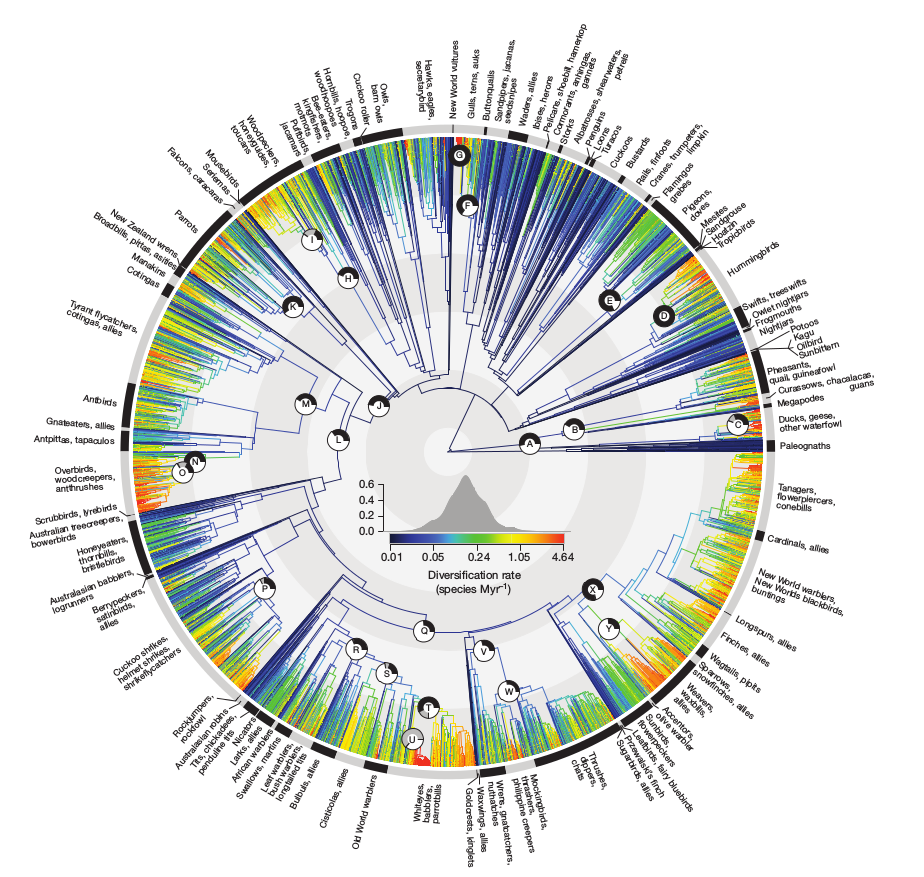
\includegraphics[scale=0.55]{Pictures/birds.png}
\caption{Diversification across the avian tree \cite{jetz2012global}. Public phylogenetic information for avian species is available in this wonderful website http://birdtree.org/.}
\label{avian}
\end{figure}




\chapter{Species Diversification}

{\color{gray} \begin{fquote}[ Alan Turing]  Mathematical reasoning may be regarded rather schematically as the exercise of a combination of two facilities, which we may call intuition and ingenuity. \end{fquote} }



\section{The evolutionary diversification process and the mechanism behind it. Review and Research Questions.}

The mechanisms behind the variation in species diversity is one of the fundamental questions of evolutionary biology. Kendall \cite{kendall1948some} considered a convenient birth-death process, which can be recast in terms of speciation and extinction events, and thus represents an extension of the Yule process \cite{yule1925mathematical}. Considering $n_t$ as the number of species (of a related genus) at time $t$, the master equation for $n_t$ in presence of extinction and speciation can be written as  

 $$ \frac{dP(n_t)}{dt} = \lambda_{n_t-1}(n_t-1)P(n_t-1)+\mu_{n_t+1}(n_t+1)P(n_t+1)-(\mu_{n_t}+\lambda_{n_t})n_tP(n_t) $$


where $\lambda_n$ and $\mu_n$ are the per capita speciation and extinction rates, respectively, and $n_t$ the total number of species on moment $t$.\\

Based on this idea, the simplest and most widely applied of a variety of model is the random speciation-extinction process \cite{nee1994reconstructed}. In a random speciation-extinction process, both speciation and extinction have instantaneous probability, or rates ($\lambda$ and $\mu$) which determine the probabilities that a clade either splits or terminates within a given time interval. In a simple branching process, the expected number of a clade increases exponentially, that is 

\begin{equation}
 E(n_t) = n_0e^{(\lambda-\mu)t} 
\label{exp1}
\end{equation}

Despite this elegance, this approach is not realistic, evolutionary history of species is widely more complex:

\begin{itemize}

	\item Each branch in the growing tree might not have the same potential fate to speciate or to get extinct. In fact, in many cases depends on several characteristics of the species.
	 
	\item Ecological interactions are important.
	
	\item Geography, location and climate influence diversification of species.
	
	\item Evolution is likely to depend on diversity of species.
	
	\item Etcetera. 

\end{itemize} 


All this ecological factors needs to be considered if we want to build model consistent with real phylogenies; for example, typically we see a common slow down on diversification towards the present \cite{moen2014does} (but see \cite{jetz2012global}) which is the opposite equation \ref{exp1} predicts. Some biological explanations might underlie diversification slowdowns, like the protracted speciation model \cite{etienne2012prolonging}, but those models do not have, for instance, a geographical component. \\

Spatial-temporal factors as well as traits and diversity dependence are some of the ecological information we should include to consider realistic models, however, this complex scenario increase the dimensionality of the system enormously, rendering them practically intractable.  \\


% Reescribir esto
%On next section we will make a quick review of the mentioned ecological factors which are potentially evolved on the mechanism underlying biodiversity and the research questions we are interested on: \\
On next chapter we will describe a novel methodological contribution to this project which aims to produce a computational feasible and consistent model selection procedure, able to take in consideration all ecological variables mentioned above. On the remaining part of this chapter we formulate and discuss the research questions this project is going to analyze. Figure \ref{Diagrama} shows a Diagram of different factors we are interested to analyze as potential drivers of species diversification; on parenthesis we recognize the research questions related to these factors. \\



%It is important to claim that we are interested in deal with interactions between species
\begin{figure}
\centering
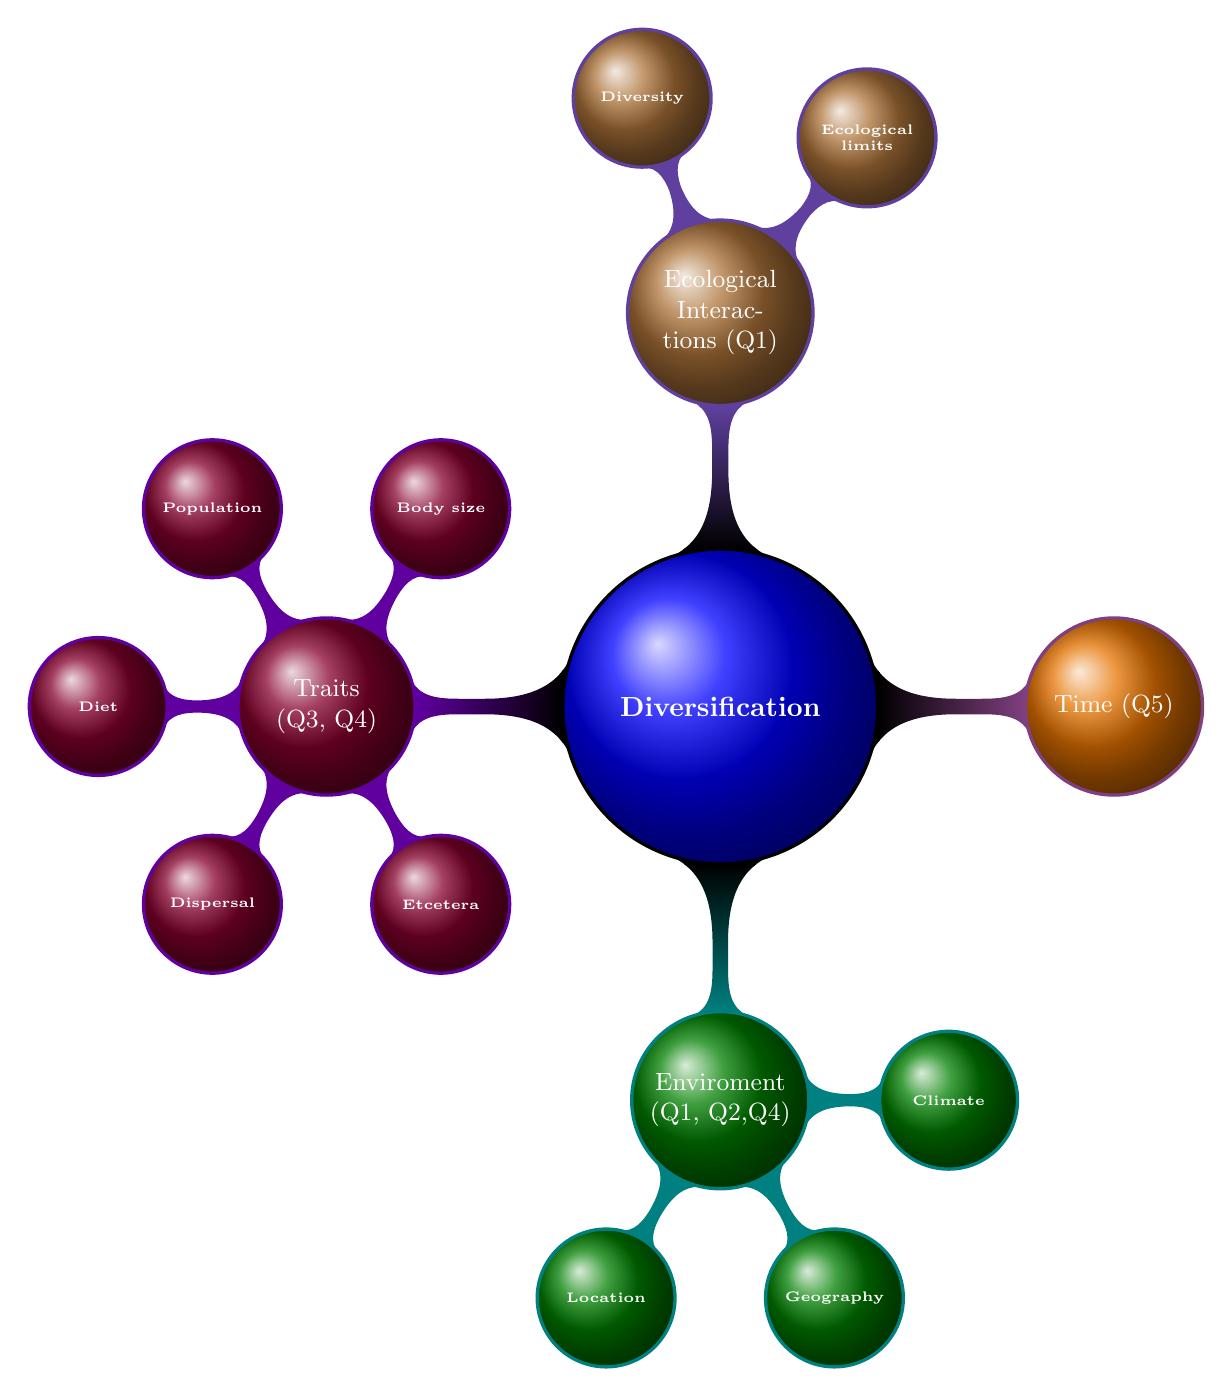
\begin{tikzpicture}
  \path [
    mindmap,
    text = white,
    level 1 concept/.append style =
      { sibling angle=90},
    level 2 concept/.append style =
      {font=\tiny\bfseries},
    level 3 concept/.append style =
      {font=\tiny\bfseries},
    tex/.style     = {concept, ball color=blue,
      font=\bfseries},
    engines/.style = {concept, ball color=green!50!black},
    formats/.style = {concept, ball color=purple!70!black},
    systems/.style = {concept, ball color=brown!90!black},
    editors/.style = {concept, ball color=orange!90!black}
  ]
  node [tex] {Diversification} [clockwise from=0]
    child[concept color=orange!50!blue, nodes={editors}] {
      node {Time (Q5)} [clockwise from=140]}	
    child[concept color=green!50!blue, nodes={engines}] {
      node {Enviroment (Q1, Q2,Q4)} [clockwise from=0]
        child { node {Climate} }
        child { node {Geography} }
        child { node {Location} }}
    child [concept color=purple!50!blue, nodes={formats}] {
      node {Traits (Q3, Q4)} [clockwise from=300]
        child { node {Etcetera} }
        child { node {Dispersal} }
        child { node {Diet} }
        child { node {Population} }
        child { node {Body size} }}
    child [concept color=brown!50!blue, nodes={systems}] {
      node {Ecological Interactions (Q1)} [clockwise from=110]
          child { node {Diversity} }
          child { node{Ecological limits} }};
\end{tikzpicture}
\caption{Representation of potential factors involved on species diversification we will include in the model. On parenthesis we see the associated research questions discussed on this chapter.}
\label{Diagrama}
\end{figure}



{\bf Q1:} Do species interaction determine diversification?\\

Species richness varies widely over the surface of the Earth \cite{ricklefs2007estimating} and patterns of species richness reflect the balance between speciation and extinction over the evolutionary history of life. Theories of how species evolve in changing environments  mostly consider single species in isolation or pairs of interacting species \cite{barraclough2015species}. \\

We are interested on the impact on interactions between species which happen locally, and therefore are hard to tackle. Reducing the complexity of the system we aim to incorporate a general approach to include species interaction on the diversification process. \\

An initial step would be to extend the approach of Etienne et al. \cite{etienne2011diversity}, which considers a caring capacity $K$ based on competition and the idea that ecological constrains place upper limits on regional diversity and that diversity is usually close to its limit \cite{cornell2013regional}. Thus, they assume that the speciation rate is limited to the caring capacity $K$ and therefore to the diversity of species $n$ 

$$ \lambda_n = \max (0, \lambda_0 - (\lambda_0 - \mu_n)\frac{n}{K} $$

We will generalize this approach considering the caring capacity $K(x)$ as a function of location $x \in \mathbb{R}^2$. Based on this, an important underlying analysis of this research question, would be to understand what is the shape of $K(x)$ as a function of location, or more generally,  the following question:\\

{\bf Q2}: How diversification rates and ecological limits varies across location?. \\


The next question is related to the impact of species' traits on diversification:\\


{\bf Q3:} Do different characteristics of species influence diversification? if yes, which ones and how they influence evolution? \\



The influence of species' traits on lineage diversification is an active area of macroevolutionary research, attributes of species, including population size, generation time, mechanism of pollination and seed dispersal, strength of sexual selection, body mass, longevity of species, diet in insects, latitude of birds and butterflies, sex allocation in flowering plants, and a large etcetera \cite{barraclough1998revealing}, has been studied and are still a matter of active research.  Sister clade comparison \cite{magallon2001absolute} has been a possible way to find relationship between traits and diversification rates, but approaches incorporating phylogenetic tree topology and the patterns of branching times had shown a greater statistical power because they incorporate more information about the patterns of diversification \cite{paradis2005statistical}. Among these methods we find models for binary-states traits \cite{maddison2007estimating},  quantitative and continuous traits \cite{fitzjohn2010quantitative}, multiple traits \cite{fitzjohn2012diversitree}, etc. But not a general approach where we can include all different kind of traits in a flexible way.


%Comparisons of species richness among sister clades enable one to test hypotheses about the influence of species attributes and environmental conditions, such as climate and landscape heterogeneity, on diversification \cite{paradis2005statistical}\\

Even though those methods have been successful finding important ecological insights in some way, they have some major drawbacks. For one side, most of the models require complete phylogenies, that is, extant specie must be present in a well-resolved phylogeny \cite{fitzjohn2009estimating}, but in reality information on extinct species is absent or, at best, incomplete; and this will never get better, simple collecting more data is not possible. For other side, even models which deals with incomplete data have a big constrain: they lack of flexibility, in the sense that they are able to be applied to very special cases, but not in a general framework, for any kind of trait. \\

It is important to note that the question Q3 is very general, and actually triggers many other research questions. For instance, dispersal is a life-history trait that influences the dynamics and persistence of populations, the distribution and abudance of species, and community structure \cite{silwood1999evolutionary}, we are also interested in their impact on evolution:\\

{\bf Q4}: What is the role of dispersal on evolutionary processes?\\



 

%We can see a decrease in diversity from its peak in the humid tropics towards higher latitudes \cite{hillebrand2004generality} \\

Finally, we would like to incorporate the temporal component on evolution as well. Several studies (e.g  \cite{rosindell2010protracted}) claim that is necessary to incorporate protracted speciation for a proper understanding of biodiversity, this makes us formulate the following question:\\


{\bf Q5}: Do we need to consider speciation as a protracted process? \\


In that way, our model should be flexible enough to incorporate protracted speciation, in the sense that it should also model speciation as a gradual process rather than an instantaneous one. \\

In this project we aim to build a general statistical framework able to incorporate any potential influential trait in a straightforward manner. Details of the methodology are described in next chapter. \\
\section{Incomplete Phylogeny trees}


A limitation of phylogenetic reconstruction based on extant species is that lineages are not represented (see Figure \ref{incomp}). This limitations makes estimating speciation and extinction rates problematic life \cite{ricklefs2007estimating}. As was mentioned before information of extinct species is usually absent or, at best, incomplete.  \\

The problem of missing data is widely considered to be the most significant obstacle in both, reconstructing phylogenetic relationships and modeling diversification process \cite{wiens2003missing}.  In this project, following Friedman et al. \cite{friedman2002structural} we will use a structural EM approach to tackle this problem efficiently. The procedure is described on next chapter.  



\begin{figure}
\centering
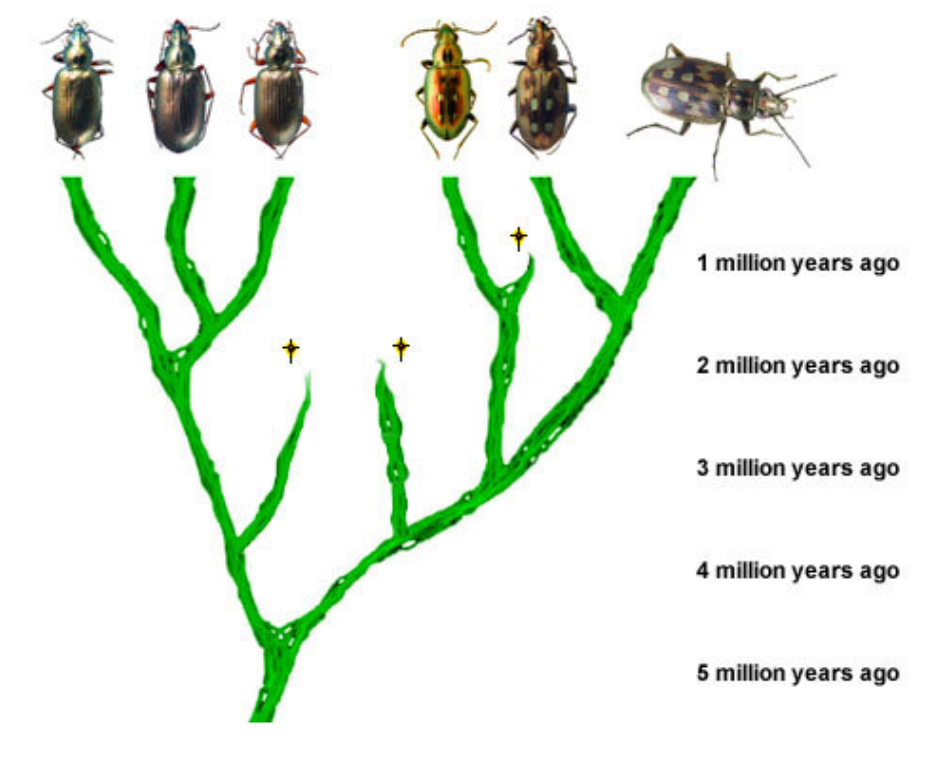
\includegraphics[scale=0.45]{Pictures/tree.png}
\caption{A phylogenetic tree of beach beetles of the genus \emph{Bembidion}. Some branches have gone extinct in the past, while others represent species living today.}
\label{incomp}
\end{figure}



\newpage
%



\chapter{Species diversification model}
{\color{gray} \begin{fquote}[Finman's Law]  Nobody wants to read anyone else's formulas. \end{fquote} }



For this chapter we will use the following notation:

%\begin{center}
%{\Large \bf Notation}
%\end{center}


\begin{description}[leftmargin=!,labelwidth=\widthof{\bfseries The longest label}]
%\item[$T$] : Time of speciation or extinction (Random Variable).
\item[$t_i$] : Branching time $i$.
\item[$n_i$] : Number of species at time $t_i$.
\item[$m$] : Number of covariates
\item[$S_i = \{ s_{i,1},...,s_{i,n_i}\}$] : Set of extant species at time $t_i$.
\item[$\lambda_{i,j}$] : Speciation rate for specie $s_{i,j}$ (at time $t_i$).
\item[$\mu_{i,j}$] : Extinction rate for specie $s_{i,j}$ (at time $t_i$).
\item[$\mathfrak{s}_i$] : Species which got speciation or extinction at time $t_i$ (note that $\mathfrak{s}_i \in S_i$ as well). 
\item[$\mathfrak{x}_1$] : Binary value; $\mathfrak{x}_i =$ "extinction" ($0$) if an extinction occurs at time $t_i$ and $\mathfrak{x}_i =$ "speciation" ($1$) if an speciation occurs at time $t_i$. 
%\item[$\pi_i$] : $\mathfrak{x}_i$ rate of specie $\mathfrak{s}_i$.  
\item[$\rho_i$] : $\mathfrak{x}_i$ rate for specie $\mathfrak{s}_i$.
\item[$x_{i,j,k}$] : $k$-covariate of the specie $j$ at time $t_i$.
\end{description}

\vspace{1cm}
\newpage
\section{Process}
We start defining the following sets: 

$$\mathcal{T} = \{t_1,...,t_p\}$$
$$\mathfrak{S} = \{\mathfrak{s}_1,...,\mathfrak{s}_p\}$$
$$\mathfrak{X} = \{ \mathfrak{x}_1, ..., \mathfrak{x}_n \} $$

The phylogenetic tree is mathematically determined by

\begin{itemize}
	\item A set of branching times $\mathcal{T}$.
	\item The topology  $\Upsilon = \{ \mathfrak{S}, \mathfrak{X} \}$.   
\end{itemize}


It is natural to assume \cite{Phyl} that the time needed for the species $s_{i,j}$ to get speciated follows an exponential distribution with parameter $\lambda_{i,j}$ and the time, of the same species, needed to get extinct follows an exponential distribution with parameter $\mu_{i,j}$. Thus, the waiting time $T_i$, defined as the minimum time, among all species, to have an speciation or extinction, also follows an exponential distribution  

	$$ P(T_i = t) = \sigma_i e^{-\sigma_i t} $$ 
	
where $\sigma_i$ is the sum of all speciation and extinction rates of extant species at time $t_i$\footnote{Note that if $X_i \sim exp(p_i)$, then $X = \min\{X_i,...,X_n\}\sim exp(\sum p_i)$. For details see \cite{casella}}. That is $\sigma_i = \sum_{j=1}^{n_i} \lambda_{i,j} +\mu_{i,j} $. \\

Moreover, given the waiting time $t_i$, the probability of speciation of the species $s_{i,j}$ is $\frac{\lambda_{i,j}}{\sigma_i}$ and the probability of extinction of the same species is $\frac{\mu_{i,j}}{\sigma_i}$.\\

		
 Then, the general version for the likelihood function of the phylogenetic tree is
 
 		\begin{equation} L( Y | \Theta) = \displaystyle\prod_{i=1}^p \sigma_i e^{-\sigma_i t_i} \frac{\rho_{i}}{\sigma_i}  
 		\label{llik}
 		\end{equation}
 		
Note that
 
\begin{itemize}
 	
 	\item $\lambda$ and $\mu$ are non-constants but functions of explanatory variables, which includes traits values, environmental phenomena, location, diversity of species or time, which makes the model fairly flexible. 
 	\item The probability of $\Upsilon$ follows a Multinomial distribution $M(n | \lambda,\mu)$ with $n=1$. However we could easily use $n > 1$ which would consider the case of multiple speciation \cite{multi}.
 	 \end{itemize}
 	 
 	

 	 
 By tacking partial derivatives equal to zero an analytical solution for \ref{llik} in the case of constant rates can be easily calculated; however, as mentioned on the previous chapter, our general (scientific) interest is to find insights of several ecological factors which could have a potential impact on the evolutionary processes of species, thus, the diversification rates are actually functions of explanatory variables
 
 %% why linear?

 $$ \lambda_{i,j} = f(\langle x_{i,j,\cdot}, \beta_1 \rangle ) $$
 $$ \mu_{i,j} = f(\langle x_{i,j,\cdot}, \beta_2 \rangle ) $$

where $\beta_1$, $\beta_2$ are $m$-dimensional vectors of parameters and $x_{i,j,\cdot}$ are $m$-dimensional vectors of ecological data (explanatory variables). $\langle \cdot, \cdot \rangle $ represents the inner product of two vectors.  \\


%On this project we will start studding the cases 
%
%\begin{itemize}
%	\item $f(x) = x$
%	\item $f(x) = e^x $
%\end{itemize}
%
%However this can be extended to any other possible biological relationship. \\
   
 For non-constant rates there is no analytical solution. We used standard optimization algorithms \cite{Bertsekas} to minimize the likelihood for three different covariates models, however, those methods are not stable. \\
 
   
 
 \section{Estimation}
 
 We are seeking for an stable and flexible method for parameter estimation and model selection. With this purpose, and considering our particular likelihood function, which has parameters which are in turn function of explanatory variables, it worth to introduce a well known statistical kind of models, the Generalized Linear Models.
 
\subsection{Generalized Linear Models}

 The unity of many statistical methods was demonstrated by Nelder and Wedderburn \cite{nelder} using the idea of the Generalized Linear Model (GLM). We present here the general set up for the Generalized Linear Model, specially applied to our research case. For a detailed study of GLM theory we refer the reader to \cite{Dobson2008} or \cite{mccullagp.j.a.nelder1989}.\\ 

Let $Y_1, Y_2, ..., Y_n$ be independent random variables, from the exponential family \footnote{For details regarding to the required mathematical assumptions concerning the exponential family of distributions we refer the reader to \cite{casella}}, and $X$ non-random matrix of explanatory variables or covariates \footnote{In our case, we are interested on potential effects of ecology factors on evolutionary processes. Then, different traits of species, climate, geographic characteristics, time and diversity of species are possible covariates of our random variable $Y$}. In general, to specify a GLM we need 

\begin{itemize}
	\item The probability distribution of $Y_i$.
	\item Equation linking the expected value of $Y_i$ with a linear combination of the explanatory variables.
	
\end{itemize} 


On this way we split the model on a random component and a systematic component, where the random component specifies the distribution of $Y_i$ and the systematic component specifies the way in which the explanatory variables comes into the model. Note that, unlike the current methods mentioned on previous chapter, we are not directly interested on estimate speciation and extinction rates itself, but we want to estimates the critical parameters which controls the underlining processes on ecological evolution. The diversification rates are functions of these parameters. 

Thus, we choose a function $g$ such that 

		$$ g(E(Y)) = \eta_i = \langle \bf{x_i}, \bf{\beta} \rangle $$
		 
where: 

\begin{itemize}

	\item $g$ is a monotone, differentiable function called the \emph{link function}.
	
	\item The vector $\bf{x}_i$ is a $m \times 1$ vector of explanatory variables.
	
	\item $\bf{\beta}$ is a $m \times 1$ vector of parameters.
	

\end{itemize}

The vector $\bf{x_i}^T$ is the $i$th row of the design matrix $\bf{X}$.\\

Note that the inference of $\beta$ is crucial in the ecological sense, as those are the indicators of relationship of ecological factors and evolutionary processes. On this project we focus our attention on the development of an efficient framework able to capture this relationship; $g(\cdot)$ expresses the relationship of the covariates as a function of $E[Y]$. \\


Summarizing, a generalized linear model has three components:

\begin{enumerate}
	\item Response variables $Y_1,...,Y_n$ from the exponential family.
	\item A set of parameters $\bf{\beta}$ and explanatory variables $\bf{X}$.
	\item monotone link function $g$ such that 	
		$$ g(E(Y_i))=\langle \bf{x}_i, \bf{\beta} \rangle $$
\end{enumerate}

%\newpage

\subsubsection{Iterative Re-Weighed Least Squares algorithm (IRWLS)}

For the estimation of parameters we use the IRWLS method [Charnes et al. 1976], which is based on the the method of scoring which in turn is based on the Newton-Raphson formula, \\

Basically, the method has the following structure:\\

 \vspace{1cm}
\fbox{%
    \parbox{12cm}{%
\begin{itemize}
	\item[i.] Obtain an initial estimate $\bf{\beta}$,
	\item[ii.] replace $f(y_i,\beta)$ with a Taylor series approximation,
	\item[iii.] evaluate all expressions that involve $\beta$ at the current estimate,
	\item[iv.]	 solve the resulting system of equations
	\item[v.] actualize the new $\beta$ and repeat (ii)-(v) until $\{ \beta^k \}$ converges.
	
\end{itemize}
}
}


.\\
\vspace{1cm}

Thus, the general formulation in the GLM context has the form,

\begin{equation} \bf{\beta}^{(m)} =  \bf{\beta}^{(m+1)} + [\mathcal{J}^{(m-1)}]^{-1}U^{(m-1)} 
\label{iterGLM}
\end{equation}

or 

\begin{equation} \mathcal{J}^{(m-1)}\bf{\beta}^{(m)} =  \mathcal{J}^{(m-1)}\bf{\beta}^{(m+1)} + U^{(m-1)} 
\label{iterGLM2}
\end{equation}


where $\bf{\beta}^{(m)}$ is the vector of estimates of the parameters $\beta_1, ... , \beta_l $ at the $m$th iteration, $[\mathbb{J}^{(m-1)}]^{-1}$ is the inverse of the information matrix and $U^{(m-1)}$ is the score function evaluated on $\bf{\beta}^{(m-1)}$. \\

Thus, we can re-write the information matrix as 

$$ \mathcal{J} = X^TWX $$

where $W$ is the diagonal matrix with elements

$$ w_{ii} = \frac{1}{Var(Y_i)}\left( \frac{\partial E(Y_i)}{\partial \eta_i} \right)^2 $$

and the expression on the right-hand side of \ref{iterGLM2} can be written as 

$$X^TW\bf{z}$$

where $\bf{z}$ has elements

$$ z_i = \langle \bf{x_i},\beta \rangle + (y_i - E(Y_i)) \left( \frac{\partial \eta_i}{\partial E(Y_i)} \right) $$

with $E(Y_i)$ and $\frac{\partial \eta_i}{\partial E(Y_i)}$ are evaluated at $\bf{\beta}^{(m-1)}$. 

Hence the iterative equation \ref{iterGLM} can be written as
%
$$X^TWX\bf{\beta}^{(m)}=X^TW\bf{z}$$
%

This is the same form as the normal equations for a linear model obtained by weighed least squares, except that it has to be solved iteratively because, in general, the components of the equation depends on $\beta$. 

\subsection{Maximun GLM likelihood for phylogenetic trees}

The implementation of the previous ideas on the phylogenetic tree has mainly two simultaneous GLM, the branching times (Br) GLM and the Topology (To) GLM. Thus, we re-write equation \ref{llik} considering both parts
 
 		\begin{equation} L( Y | \Theta) = \displaystyle\prod_{i=1}^p \displaystyle\underbrace{\sigma_i e^{-\sigma_i t_i}}_{Bt} \displaystyle\underbrace{\rho_i / \sigma_i}_{To}  
 		\label{llik2}
 		\end{equation}
 		
and we are looking for the log-likelihood function

$$ l(\beta) = l^{Bt}(\beta) + l^{To}(\beta) $$
 		
 Our aim is to find the MLE of \ref{llik}, that is
 
 
 $$ \hat{\beta} = \displaystyle\argmax_{\beta} l(\beta) = \displaystyle\argmax_{\beta} l^{Bt}(\beta) + l^B(\beta)$$ 
 
 
Then, for the whole phylogeny we consider 

$$X^TWX = X^{Bt}W^{Bt}X^{Bt} + X^{To}W^{To}X^{To} $$
 
thus, our iterative procedure corresponds to 
\begin{equation}
  X^T W X\beta^{(m)}=X^TW\bf{z}
  \label{iter}
\end{equation}
 where
 
 \[
X=
  \begin{bmatrix}
    X^{Bt} \\
   X^{To}
  \end{bmatrix},
\]

\[
W =
  \begin{bmatrix}
    W^{Bt}   &  0 \\
    0 &  W^{To} 
  \end{bmatrix}
\]
and 
  \[
Z=
  \begin{bmatrix}
    Z^{Bt} \\
   Z^{To}
  \end{bmatrix}
\]


thus, to performs the MLE minimization we need the formulation of $$X^{Br}, W^{Br}, Z^{Br}, X^{To}, W^{To}, Z^{To}.$$  

\subsubsection*{The branching times (Bt)}
	
As mentioned before, $T_i$ follows an exponential distribution 
	
	$$ P(T_i = t_i) = \sigma_i e^{-\sigma t_i} $$
	
thus 

\begin{equation}
E(T_i) = \frac{1}{\sigma_i}  \text{ and } Var(T_i) = \frac{1}{\sigma_i^2}
\label{espvar1}
\end{equation}


By other side, we have 

%$$ \sigma_i = \displaystyle\sum_{j=1}^{n_j} \rho_{i,j} =  \displaystyle\sum_{j=1}^{n_j} \langle x_{i,j}, \beta \rangle = \langle \sum_j x_{i,j} , \beta \rangle = \langle \bf{x}_i , \beta \rangle $$

\begin{align*}
\sigma_i &= \displaystyle\sum_{j=1}^{n_i} \lambda_{i,j} + \mu_{i,j} \\
	     &= \displaystyle\sum_{j=1}^{n_i} \langle x_{i,j,\cdot}, \beta_1 \rangle + 				\langle x_{i,j,\cdot}, \beta_2 \rangle \\
	     &= \langle \sum_j x_{i,j,\cdot}, \beta_1 + \beta_2 \rangle \\ 
	     &= \left\langle \bf{x}_i^{Bt} , \beta^{Bt} \right\rangle 
\label{linear}
\end{align*}


%
then, by \ref{espvar1}, the equation above, and following the GLM procedure, we get the link function $g(x) = 1/x$. \\

we use this to calculate the matrix $W$, 

$$ w_{ii}^{To} = \frac{1}{Var(T_i)}\left( \frac{\partial E(T_i)}{\partial \eta_i} \right)^2 $$

where, $Var(T_i)$ is given by \ref{espvar1} and 

$$ \frac{\partial E(T_i)}{\partial \eta_i} = \frac{\partial g^{-1}(\eta_i)}{\partial \eta_i} = \frac{\partial \frac{1}{\eta_i}}{\partial \eta_i} = -\frac{1}{\eta_i^2} = -\frac{1}{\left\langle \bf{x}_i , \bf{\beta} \right\rangle ^2} $$ 

Then, $$w_{ii} = 1/\langle \bf{x}_i , \beta \rangle ^2, \forall i$$
Thus, 

\[
W^{Bt}=
  \begin{bmatrix}
    1/\sigma_1     &      0 & \cdots &  0 \\
     0     &     1/\sigma_2 & \ddots &  0 \\
    \vdots & \ddots & \ddots  & 0 \\
     0     &      0 & 0 &  1/\sigma_p 
  \end{bmatrix}
\]

%Following the GLM procedure, let $g(x)$ be a real function such that 
%$$ g(E(T_i)) = g(\frac{1}{\sigma_i})  = \langle \bf{x}_i , \beta \rangle  $$   

%then, $g(x) = 1/x$ 


Moreover, 

$$
 z_i^{Bt}  = \langle {\bf x_i},\beta \rangle + (t_i - E(T_i)) \left( \frac{\partial \eta_i}{\partial E(T_i)} \right)  = \sigma_i(2-t_i\sigma_i)
$$



Then, we could compute the IRWLS iterations for the exponential distribution case


$$(X^{Bt})^TW^{Bt}X^{Bt}\bf{b}^{(m)}=(X^{Bt})^TW^{Bt}\bf{z}^{Bt}$$

where 

\[
X^Bt=
  \begin{bmatrix}
    \sum_j x_{1,j,1}     &   \sum_j x_{1,j,2} & \cdots &  \sum_j x_{1,j,m} \\
    \sum_j x_{2,j,1}     &   \sum_j x_{2,j,2} & \ddots &  \sum_j x_{2,j,m} \\
    \vdots & \ddots & \ddots  & \vdots \\
     \sum_j x_{p,j,1}     &      \sum_j x_{p,j,2} & \cdots &  \sum_j x_{p,j,m} 
  \end{bmatrix}
\]

with $x_{i,j,k}$ is the $k$-covariate for the specie $j$ at time $t_i$. \\



%This is half of our log-likelihood function, let's check the multinomial part


\subsubsection*{The topology}


 As described previously the topology $\Upsilon_i$ follows a multinomial distribution \\ $MN(1,\lambda_1,\mu_1,\lambda_2,\mu_2,...,\lambda_{n_i},\mu_{n_i})$, \\
 
 
 for convenience, we define $\pi_i=\frac{\rho_i}{\sigma_i}$, where $\rho_i$ is the $\mathfrak{x}_i$ rate of the specie $\mathfrak{s}_i$ \footnote{Note that $\mathfrak{x}_i$ is a string corresponding to "speciation" or "extinction", please see the notation section for details.}. In other words, $\pi_i$ is the probability that the specie $\mathfrak{s}_i$ evolves at time $t_i$ as had happened.
 
 Then, we define the Bernoulli distributed random variable $Z_i \sim B(\pi_i) $, \\
 
note that 

$$ l^{To}=L(Z_i|\pi) = \displaystyle\prod_{i=1}^n \pi_i $$

and $E[Z_i] = \pi_i$,        $Var(Z_i) = \pi_1(1-\pi_i)$
	
then, we can work with $Z_i$ instead of $\Upsilon_i$ as they have same Likelihood function. 

we can $\pi_i$ this as 

$$ \pi_i = \frac{\eta_i}{\eta_i + c_i} $$ 

where $\eta_i = \langle x_{i,\mathfrak{s}_i},\beta \rangle $ and $c_i = \langle \displaystyle\sum_{j\neq \mathfrak{s}_i}^{n_i} x_{i,j}, \beta \rangle $. Thus, 

$$ \eta_i^{To} \frac{1}{c_i} = \frac{\pi_i}{1-\pi_i} $$ 

and 
 $$g(\pi_i) = \frac{\pi_i}{1-\pi_i} $$ 
	
then, 	
	% caminar por las calles de paris me recuerda la cuidad de mi amor <3... por el olor a meao nomas si, por que valpo es infinitamente mas maravilloso que paris :).
	\[
X^{To}=
  \begin{bmatrix}
 	x_{1,\mathfrak{s_1},1} & x_{1 , \mathfrak{s}_1 , 2} & \cdots & x_{1,\mathfrak{s}_2,m} \\
 	x_{2,\mathfrak{s_2},1} & x_{2,\mathfrak{s}_2,2} & \cdots & x_{2,\mathfrak{s}_2,m} \\
 	\vdots & \ddots & \cdots & \vdots \\
 	x_{p,\mathfrak{s_p},1} & x_{p,\mathfrak{s}_p,2} & \cdots & x_{p,\mathfrak{s}_p,m} \\
  \end{bmatrix}
\]


$$w_{ii}^{To} = \frac{1}{\pi_i(1-\pi_i)}\frac{c_i^2}{(\eta_i+c_i)^4} = c_i\pi_i^2$$

and

\[
W^{To}=
  \begin{bmatrix}
    c_1\pi_1^2     &      0 & \cdots &  0 \\
     0     &    c_2\pi_2^2 & \ddots &  0 \\
    \vdots & \ddots & \ddots  & 0 \\
     0     &      0 & 0 & c_p\pi_p^2
  \end{bmatrix}
\]

moreover, 

$$ z_i^{To} = \displaystyle\sum_{k=1}^m x_{i,\mathfrak{s}_i,k} \beta_k + \frac{\pi_ic_i^2}{(1-\pi_i)^3} $$
	
	
then, $Z^{To} = [z_1^{To},...,z_p^{To}]^T$.


 \subsubsection*{The phylogenetic tree (branching times + topology)}
 
 Finally, we have $$X^{Br}, W^{Br}, Z^{Br}, X^{To}, W^{To}, Z^{To}.$$ With this we can perform the equation \ref{iter} iterativelly.
 
 
%% Our aim is to find the MLE of \ref{llik}, that is
%% 
%% 
%% $$ \hat{\beta} = \displaystyle\argmax_{\beta} l(\beta) = \displaystyle\argmax_{\beta} l^G(\beta) + l^B(\beta)$$ 
%% 
%% 
%%Then, for the whole phylogeny we consider 
%%
%%$$X^TWX = X^{Bt}W^{Bt}X^{Bt} + X^{To}W^{To}X^{To} $$
%% 
%%Or, 
%% 
%%
%% 
%% 
%% $$X^TWX\bf{b}^{(m)}=X^TW\bf{z}$$
%% 
%% where
%% 
%% \[
%%X=
%%  \begin{bmatrix}
%%    X^G \\
%%   X^B
%%  \end{bmatrix}
%%\], 
%%
%%\[
%%W =
%%  \begin{bmatrix}
%%    W^G   &  0 \\
%%    0 &  W^B 
%%  \end{bmatrix}
%%\]
%%and 
%%  \[
%%Z=
%%  \begin{bmatrix}
%%    Z^G \\
%%   Z^B
%%  \end{bmatrix}
%%\]

%\subsection{Some prior results}

%\newpage


\subsubsection{Example 1: Diversity-dependence model }

As a first example we formulate a diversity-dependence model \cite{etienne2011diversity}, where the speciation rate depends linearly on the number of species $n_i$ and the extinction rate is constant, 

$$ \lambda_{i,j} = \lambda_0 - (\lambda_0 - \mu_0)\frac{n_i}{K}, \qquad \mu_n = \mu_0 $$ 


where $\lambda_0$, $\mu_0$ and $K$ are the parameters corresponding to initial speciation rate, extinction rate and carrying capacity respectively. \\

Note that this model assumes equal rates for different species, or in other words, all topologies are equally probable.The log-likelihood function has the form 

$$  l = \sum_{i=1}^p ln(\sigma_i) - \sigma_i t_i + ln\left(\frac{1}{n_i}\right) $$

where 

\begin{equation}
\begin{aligned}
 \sigma_i & = \sum_{j=1}^{n_i}  \lambda_0 - (\lambda_0 - \mu_0)\frac{n_i}{K} + \mu_0 \\
 		& = n_i(\lambda_0 + \mu_0) - n_i^2\left(\frac{\lambda_0-\mu_0}{K}\right) \\
 		& = \langle x_i^{Bt}, \beta^{Bt} \rangle = \eta_i \end{aligned} \end{equation}
 		
 	%= \frac{1}{E[T_i]} 
 	
 where
$$ 
 x_i^{Bt}=
  \begin{bmatrix}
    n_i \\
   n_i^2
  \end{bmatrix}, \qquad \beta^{Bt}=
  \begin{bmatrix}
    \beta_1 \\
   \beta_2
  \end{bmatrix} =   \begin{bmatrix}
    \lambda_0+\mu_0\\
   \frac{\mu_0-\lambda_0}{K}
  \end{bmatrix}
$$ 

then, 

$$ \frac{\partial E[T_i]}{\partial \eta_i} = \frac{\partial (1/ \sigma_i)}{\partial \sigma_i} = -\frac{1}{\sigma_i^2}$$

and

$$ \frac{\partial \eta_i}{\partial E[T_i]} = \frac{\partial (1/E[T_i])}{\partial E[T_i]} = -\frac{1}{E^2[T_i]} = -\sigma_i^2 $$

thus, 

$$ w_{ii}^{Bt} = \sigma_i^2 \frac{1}{\sigma_i^4} = \frac{1}{\sigma_i^2} $$ 

and

\[
W^{Bt} = \left(
 \begin{array}{ccccc}
   \frac{1}{\sigma_1^2}\\
    & \ddots & & \text{\huge0}\\
    & & \ddots\\
    & \text{\huge0} & & \ddots\\
    & & & & \frac{1}{\sigma_p^2}
 \end{array}
\right)
\]

moreover, 

$$ z_i^{Bt} = n_i(\lambda_0 + \mu_0) + n_i^2\frac{\mu_0-\lambda_0}{K} - (t_i -\frac{1}{\sigma})\sigma_i^2 $$


then 

$$\bf{z}^{Bt} = \begin{bmatrix}
     n_1(\lambda_0 + \mu_0) + n_1^2\frac{\mu_0-\lambda_0}{K} - (t_1 -\frac{1}{\sigma_1})\sigma_1^2 \\
   \vdots \\
  n_p(\lambda_0 + \mu_0) + n_p^2\frac{\mu_0-\lambda_0}{K} - (t_p -\frac{1}{\sigma_p})\sigma_1^2
  \end{bmatrix}
$$

and
$$ 
 X^{Bt}=
  \begin{bmatrix}
    n_1 &   n_1^2 \\
    \vdots & \vdots \\
    n_p & n_p^2
  \end{bmatrix}
$$ 


Finally, with all these values we are ready to run the following iterative procedure which will find the MLE parameter estimator 

$$\beta^{(m)}=[(X^{Bt})^TW^{Bt}X^{Bt}]^{-1}(X^{Bt})^TW^{Bt}\bf{z}^{Bt}$$

Note that the right side of the equation above depends on $\beta$, so we choose $\beta_0$ and then we replace $\beta$ with the previous calculated beta on each iteration. \\

This is the simplest model for diversity dependence, however this model does not account for geographic variables, and does not even use topology information. We aim to generalize it considering location information and incorporating traits dependence, under the GLM approach this extension is quite straightforward.  

 
\subsubsection{Example 2: Linear model for traits dependence}

As a second example, we generalize the linear model for traits dependence \cite{paradis2005statistical} including a non-constant extinction rate. The relation of body mass and diversification rates have been studied with different approaches \cite{gittleman1998body}, based on that we formulate diversification rates as

$$ \lambda_{i,j} = \beta_0 +\beta_1 ln(body mass_{i,j})= \beta_0 + \beta_1 v_{i,j} $$ 
$$ \mu_{i,j} = \beta_3 +\beta_4 ln(body mass_{i,j}) = \beta_2 + \beta_3 v_{i,j}$$

Here we define $v_{i,j}$ as the log of the body mass of specie $j$ at time $t_i$, then for the branching times formulation we calculate 

\begin{equation}
\begin{aligned}
 \sigma_i & = \displaystyle\sum_{j=1}^{n_i} \lambda_{i,j} + \mu_{i,j} \\
 & n_i(\beta_0 + \beta_2) + \left[ \displaystyle\sum_{j=1}^{n_i} v_{i,j} \right](\beta_1 + \beta_2) \\
 & = \langle x_i^{Bt}, \beta^{Bt} \rangle = \eta_i^{Bt} \end{aligned} \end{equation} 

where

$$ 
 x_i^{Bt}=
  \begin{bmatrix}
    n_i \\
  \displaystyle\sum_{j=1}^{n_i} v_{i,j}
  \end{bmatrix}, \qquad \beta^{Bt}=
  \begin{bmatrix}
    \beta_0 + \beta_2 \\
   \beta_1 + \beta_3 \end{bmatrix}
$$ 

moreover, we have 

\[
W^{Bt} = \left(
 \begin{array}{ccccc}
   \frac{1}{\sigma_1^2}\\
    & \ddots & & \text{\huge0}\\
    & & \ddots\\
    & \text{\huge0} & & \ddots\\
    & & & & \frac{1}{\sigma_p^2}
 \end{array}
\right),
\]

$$\bf{z}^{Bt} = \begin{bmatrix}
     n_1(\beta_0 + \beta_2) + \left( \displaystyle\sum_{j=1}^{n_1} v_{1,j} \right)(\beta_1 + \beta_2) +(t_1-1/ \sigma_1)\sigma_1^2\\
   \vdots \\
  n_p(\beta_0 + \beta_2) + \left( \displaystyle\sum_{j=1}^{n_p} v_{p,j} \right)(\beta_1 + \beta_2) +(t_p-1/ \sigma_p)\sigma_p^2
  \end{bmatrix}
$$

and
$$ 
 X^{Bt}=
  \begin{bmatrix}
    n_1 &    \displaystyle\sum_{j=1}^{n_1} v_{1,j} \\
    \vdots & \vdots \\
    n_p &  \displaystyle\sum_{j=1}^{n_p} v_{p,j}
  \end{bmatrix}
$$ 

For the topology part we consider

$$ \pi_i = \frac{\rho_i}{\sigma_i} = \frac{(\beta_0+\beta_1 v_{i,\mathfrak{s}_i})\mathds{1}(\mathfrak{x_i})+(\beta_2+\beta_3v_{i,\mathfrak{s}_i})(1-\mathds{1}(\mathfrak{x_i})) }{n_i(\beta_0+\beta_2)+(\sum_j^{n_i} v_{i,j})(\beta_1+\beta_3)} $$

where

$$ \mathds{1}(\mathfrak{x_i}) =\left\{ \begin{aligned} 1 &\qquad if & \mathfrak{x_i} = "speciation" \\
0 & \qquad if & \mathfrak{x_i} = "extinction" 
 \end{aligned} \right. $$

then, following the procedure described on previous chapter, we re-write $\pi_i$ on the form 

$$ \pi_i = \frac{\rho_i}{\rho_i + c_i} $$

where $c_i = \sigma_i - \rho_i$. moreover, 

$$\begin{aligned} \rho_i & = \beta_0  \mathds{1}(\mathfrak{x_i})  + \beta_1 v_{i,\mathfrak{s}_i}  \mathds{1}(\mathfrak{x_i}) + \beta_2 + \beta_3v_{i,\mathfrak{s}_i} - \beta_2 \mathds{1}(\mathfrak{x_i})-\beta_3v_{i,\mathfrak{s}_i} \mathds{1}(\mathfrak{x_i}) \\
& = \langle x_i^{To},\beta^{To} \rangle = \eta_i^{To} \end{aligned}  $$

where, 

$$ 
 x_i^{To}=
  \begin{bmatrix}
    \mathds{1}(\mathfrak{x_i}) \\
    v_{i,v_{i,\mathfrak{s}_i}}\mathds{1}(\mathfrak{x_i}) \\
    1 \\
    v_{i,v_{i,\mathfrak{s}_i}}
  \end{bmatrix}, \qquad
 \beta^{To} =
 	\begin{bmatrix}
 		\beta_0 - \beta_2 \\
 		\beta_1 - \beta_3 \\
 		\beta_2 \\
 		\beta_3
 	\end{bmatrix}
$$ 
and 


\[
W^{To}=
  \begin{bmatrix}
    c_1\pi_1^2     &      0 & \cdots &  0 \\
     0     &    c_2\pi_2^2 & \ddots &  0 \\
    \vdots & \ddots & \ddots  & 0 \\
     0     &      0 & 0 & c_p\pi_p^2
  \end{bmatrix}
\]

moreover, 

$$ z_i^{To} = \displaystyle\sum_{k=1}^m x_{i,\mathfrak{s}_i,k} \beta_k + \frac{\pi_ic_i^2}{(1-\pi_i)^3} $$
	
	
then, $Z^{To} = [z_1^{To},...,z_p^{To}]^T$.

 With all these values we perform iteratively the following equation 
 
 $$\beta^{(m)}=[(X^{Bt})^TW^{Bt}X^{Bt}]^{-1}(X^{Bt})^TW^{Bt}\bf{z}^{Bt}$$
 
 \subsubsection*{Discussion}
 
 
As we can see, this method allows easy generalization to important extensions on ecology: 

\begin{itemize}
	\item We can include any kind of multiple traits, quantitative and continuous, binary traits (using identity functions), geographical variables like range of species, etcetera. 
	\item We can also study migration influences including on the link function of the GLM. 
	\item As mentioned before we can extend to the case of multiple speciation allowing the multivariate distribution to have parameter $n>1$.
	\item We can include protracted speciation adding an additional parameter to the exponential distribution.
	
\end{itemize} 
 
 
Most of the data is indeed incomplete. To overcome this statistical problem we introduce the well known Expectation Minimization algorithm in next section. 
 
\subsection{Incomplete phylogenetic trees. The EM algorithm}

As discussed on the introductory chapter, in evolutionary ecology, or more specifically, on phylogenic trees, we are actually full of missing observations since we can only observe extant species with molecular data and fossil record is very poor and most of the time absent. Then, the described model is not really enough to afford real data. 

In statistics, an expectation-maximization (EM) \cite{em} algorithm is an iterative method for finding MLE of parameters in statistical models, where the model depends on unobserved latent variables. 


 More formally, we consider $\mathcal{Y} = \{\tau_{obs},\Upsilon_{obs}\}$ as the tree containing observed branching times and topology of the tree. In a similar way we define $y_{miss} = \{\tau_{mis},\Upsilon_{mis}\}$ as the "missing part" of the real phylogenetic tree, that is information of extinct species not included in current data. Finally we define the real phylogenetic tree of a clade as $\mathcal{Z} = \mathcal{Y} \cup y_{miss}$. \\
 
We then define the $Q$ function as the expectation of the log-likelihood function 
 
 $$ Q(\beta,\beta_0) = \int_{Y_{miss}} log(p(\beta | y_{miss}, \mathcal{Y}))p(y_{miss} | \beta_0, \mathcal{Y}) dy_{miss} $$
 

Where $Y_{miss}$ is the (infinite) set of all possible latent trees, or missing part of the real tree. Then $y_{miss} \in Y_{miss}$ is a variable, and $Q$ is an integral along all possible values of $y_{miss}$. In this way, given the current approximation to the maximizer of the observed posterior ($\beta^{(i)}$), the E step of the EM algorithm is defined by computing

\begin{equation}
 Q(\beta,\beta^{(i)})=\int_{Y_{miss}} log(p(\beta | y_{miss},\mathcal{Y}))p(y_{miss} |\beta^{(i)},\mathcal{Y})dy_{miss} 
 \label{em1}
 \end{equation}

The M step then corresponds to maximize the $Q$ function with respect to $\beta$ to obtain the update $\beta^{(i+1)}$. \\

In the case of phylogenetic trees, the calculation of \ref{em1} is not straightforward since $p$ has the form of equation \ref{llik2}. To perform this integration we use the Monte Carlo EM(MCEM) algorithm \cite{mcem}. The general structure is as follows

 \vspace{1cm}
\fbox{%
    \parbox{12cm}{%
\begin{itemize}
	\item[i.] Obtain an (initial) estimate $\beta^{(i)}$,
	\item[ii.] generate a sample $y_{miss}^{(1)}, ...,y_{miss}^{(h)}$ from the current approximation to the conditional predictive distribution $p(y_{miss}|\beta^{(i)},\mathcal{Y})$,
	\item[iii.] update the current approximation to $Q_{i+1}(\beta,\beta^{(i)})$, to be the mixture of augmented log-posteriors of $\beta$, mix over the latent data patterns from (ii)
	$$ Q_{i+1}(\beta,\beta^{(i)}) = \frac{1}{N} \displaystyle\sum_{j=1}^N log(p(\beta | y_{miss}^{(j)},\mathcal{Y}))$$
	\item[iv.] the M step corresponds to the maximization of the right side of the equation above. 
	\item[v.] update the conditional predictive distribution, actualize the new $\beta$ and repeat (ii)-(v) until convergence.
	
\end{itemize}
}
}



\subsection{Automatic selection of variables: differential geometric extension of the least angle regression method.}

So far, we have described the mathematical methodology for inference of parameters based on incomplete phylogenies. However, as mentioned on previous chapter, the complexity of the problem is just huge, we need to deal with an enormous amount of ecological and complex information which will be almost impossible to handle with the structural EM algorithm itself. To make this framework feasible we embed a differential geometric path finding method \cite{augugliaro2013differential} inside the M-step if the EM algorithm. This will produce a sparse, computationally feasible and consistent model selection procedure. \\


As defined previously $\mathcal{Y}$ as the observed phylogenetic tree, and $\mathcal{Z}$ indicates the complete phylogenetic tree (see figure \ref{incomp}). Then, the the $q$-th score function, measuring the likelihood increase in the $q$-th direction is given by 

	$$ \partial_q l(\beta;y) = \frac{\partial log(p(y;\beta))}{\partial \beta_q}$$
	
	
To measure the scale of this change, relative to the size of the $q$-th predictor, we scale the score function by the square root of the conditional Fisher information, i.e $I_q(\beta) = \partial^2 l(\beta ; y) / \partial \beta^2_q $ to obtain the conditional Rao score statistic, 

$$ r_q^u (\beta) = \frac{\partial_q l(\beta ; y)}{\sqrt{I_q(\beta)}} $$

We can note that, under regularity conditions, at the maximum likelihood estimate the Rao score statistic is equal to zero, since the derivatives of the likelihood are zero. \\

On the other hand, for an initial estimate $\hat{\beta}_0$, for instance $\hat{\beta}_0 = (b_0,0,...,0)$, we define $\gamma_{max}$ to be the largest absolute value of the Rao score statistic at $\hat{\beta}_0$ 

	$$ \gamma_{max} = \displaystyle\max_{q=1,...,m} |r_q^u(\hat{\beta}_0)|$$

This value points out the best instantaneous normalized contribution to the likelihood of a single variable. This particular variable would make an excellent candidate for being included in the model. With these definitions in hand, we can now define the model extension estimator. \\

Let $\gamma \in [0,\gamma_{max} ]$ be a fixed value. The model extension estimator of a given spatial birth-death model, denoted by $\hat{\beta}(\gamma) \in \mathbb{R}^m$, is such that the following conditions are satisfied: 

	$$ |r_q^u (\hat{\beta}(\gamma))| = \gamma, \qquad \forall q \in \mathcal{A}(\gamma)$$
	$$ |r_q^u (\hat{\beta}(\gamma))| < \gamma, \qquad \forall q \notin \mathcal{A}(\gamma)$$


where $\mathcal{A}(\gamma) = \{ m:\hat{\beta}_q(\gamma) \neq 0 \}$ is called active model set. \\

Here we have defined the model extension estimator in terms of the Rao score statistic. Augugliaro et al. \cite{augugliaro2013differential} shows that the conditions above follow naturally from a differential geometric interpretation of a model, which allows us to generalize the least angle regression method (LARS) introduced in Efron et al \cite{efron2004least}. The new method generalized the geometric description of LARS and is based on the following simple differential geometric identity 

	$$ r_q^u (\beta) = cos \rho_q (\beta) \cdot \| r_{\beta} (\mathcal{Y}) \|_{p(E(\beta))} $$
	
	where in this case $\rho_q(\beta)$ is the angle between $\partial_q l(\beta;\mathcal{Y})$ and the tangent residual vector $r_{\beta}(\mathcal{Y})$ while  $\| r_{\beta} (\mathcal{Y})\|_{p(E(\beta)}$ is the length of this vector -- which, crucially, does not depend on variable $q$. Using figure \ref{dglars} the dgLARS method can be described in the following way. First the method selects the predictor, say $\mathcal{X}_{a_1}$, whose basis vector $\partial_{a_1} l(\hat{\beta}(\gamma_{max});\mathcal{Y})$ has the smallest angle with the tangent residual vector, and includes it in the active set $\mathcal{A}(\gamma^{(1)} = \{ a_0, a_1 \}$, where $a_0$ stands for the intercept and $\gamma^{(1)} = \gamma_{max}$. The solution curve $\hat{\beta} (\gamma) = (\hat{\beta}_{a_0}(\gamma), \hat{\beta}_{a_1}(\gamma),0,...,0)^T$ is chosen in such a way that the tangent residual vector is always orthogonal to the basis $\partial_{a_0}l(\hat{\beta}(\gamma);\mathcal{Y})$, while the direction of the curve $\hat{\beta}(\gamma)$ is defined by the projection of the tangent residual vector onto the basis vector $\partial_{a_1} l(\hat{\beta}(\gamma);\mathcal{Y})$. The curve $\hat{\beta}(\gamma)$ continues as defined above until $\gamma^{(2)} < \gamma^{(1)}$, for which there exists a new predictor, say $\mathcal{X}_{a_2}$, that satisfies the equiangularity condition, namely 
	
	\begin{equation} \rho_{a_1}(\hat{\beta}(\gamma^{(2)})) = \rho_{a_2}(\hat{\beta}(\gamma^{(2)})) \label{le} \end{equation}
	
At this point $\mathcal{X}_{a_2}$ is included in $\mathcal{A}(\gamma^{(2)})$ and the curve $$\hat{\beta}(\gamma) = (\hat{\beta}_{a_1}(\gamma),\hat{\beta}_{a_1}(\gamma),\hat{\beta}_{a_2}(\gamma),0,...,0)^T$$ continues, such that the tangent residual vector is always orthogonal to the basis vector $\partial_{a_1} l(\hat{\beta};\mathcal{Y})$ and $\partial_{a_2} l(\hat{\beta}(\gamma);\mathcal{Y})$, as shown on the right side of figure \ref{dglars}.\\

At the end, model reduction requires selecting a tuning parameter $\hat{\gamma}$ that controls the sparsity or shrinkage of the model. Especially in complex models, like this one, it is important to tune this inference to the available data \cite{wit2012all}. For that purposes we will adjust the fast generalized cross-validation and generalized information criterion \cite{abbruzzo2014generalized} \cite{2013arXiv1309.6216V} adjusted to phylogenetic trees.

\begin{figure}
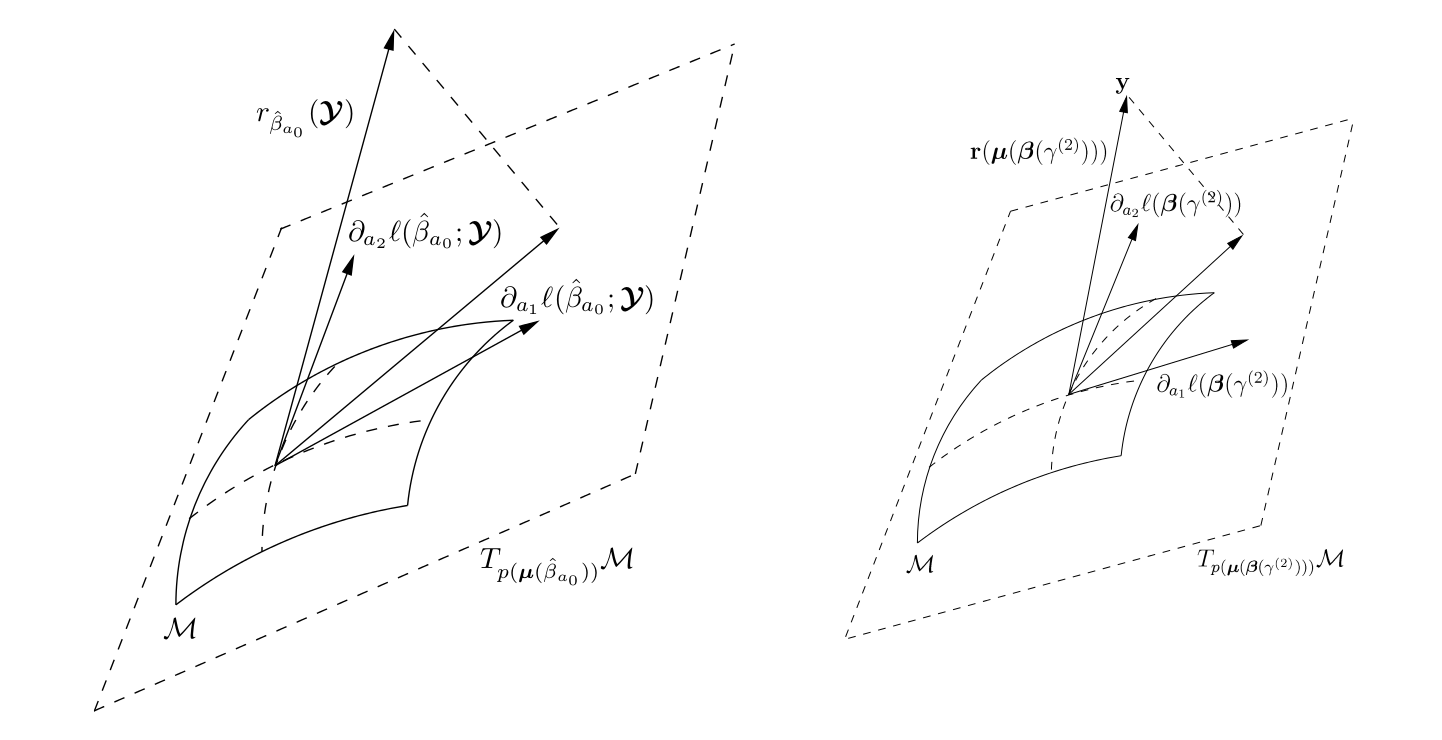
\includegraphics[scale=0.4]{Pictures/diff.png}
%\caption{jo $x$}
\caption{Differential geometrical description of the model extension method for birth-death speciation model with two covariates; in the left side the first predictor $\mathcal{X}_{a_1}$ is found and included in the active set; in the right side the generalized equiangularity condition \ref{le} is satisfied for $\mathcal{X}_{a_1}$ and $\mathcal{X}_{a_2}$ \cite{augugliaro2013differential}}
\label{dglars} 
\end{figure}



 
\newpage

\chapter{Knowledge utilization}




\section{Implementation of results}


\subsection{Software development}
We will develop free software packages for the often mathematically and computationally demanding inference techniques, allowing non-specialist scientist to apply these newly developed methods easily to their own systems.


\subsection{Application to real data}

We will test the methods on published phylogenies, but also on a new phylogeny of microlandsnails on limestone outcrops on Malaysian Borneo that will be constructed in research funded by a VICI grant awarded to R.S. Etienne. This system is unique in that contains well-defined local communities (the snails are strongly restricted to the limestone) with limited dispersal and high endemism. Besides contituting a miniature world ideally suited for trying out our new methods, the microsnail ecological evolutionary dynamica is a real life system that can reveal the effects of global warming on biodiversity.

\section{Contribution of research to specific fields beyond mathematics, ecology and evolution: Language evolution}

Phylogenetic methods are increasingly used to study language evolution. This project can help identify the phylogeographic context and the influence of community effects (e.g number of languages present) on language diversification in different human societies. We will collaborate with Quentin Atkinson (University of Auckland) and localized evolution models are also there an important inferential hurdle that has not been taken yet.

\section{Contribution of research to society: Global conservation} 

Understanding the processes driving biodiversity is of crucial importance for assessing the effects of global change on the diversity of life on this planet. This project will help addressing the following key issues: (1) if local diversity limits further diversification, will a reduction in diversity then speed up diversification and restore the balance, and if so, over what time scale will equilibrium be recovered; or (2) will lost diversity never be regained, because the loss happens too quickly for natural processes to compensate?

\section{Open Access policy}

Scientific publications arising from this project will be made publicly accessible to the research community, by depositing submitted/accepted manuscripts at arXiv.org and choosing Open Access journals options. This will allow the unconditional and immediate availability of the scientific results for use by other scientist and general public, particularly in developing countries. 
\newpage
\chapter{Time Planning}

\begin{table}[h!]
%\caption{Timeline.}
%\centering
%\begin{minipage}[t]{\linewidth}
\color{gray}
\rule{\linewidth}{1pt}
\ytl{2016 May - 2017 Apr}{{\bf Project 1:} Spatial birth-death model of diversification. \\ {\bf Deliverable:} Paper}
\ytl{2017 May - 2018 Apr}{{\bf Project 2:} Robust inference of spatial diversification. \\ {\bf Deliverable:} Paper, R package (version 1). Organize statistical workshop on geographical dynamics of speciation.}
\ytl{2018 May - 2019 Apr}{{\bf Project 3:} Geographic dynamics of speciation events in real applications. \\ {\bf Deliverable:} Paper, R package (version 2)}
\ytl{2019 May - 2019 Oct}{Complete PhD thesis. \\ {\bf Deliverable:} Thesis.}

\bigskip
\rule{\linewidth}{1pt}%
%\end{minipage}%
\end{table}
%\thispagestyle{fancy}
%\mbox{}
\newpage

\bibliography{Bibliography} 
%\bibliographystyle{ieeetr}
\bibliographystyle{apalike}


\end{document}

